% Исследовательская часть
\section{Исследовательская часть}

\hspace{1.25cm}
Для сравнения времени реализаций стандартного алгоритма, алгоритма Винограда и его оптимизированной версии программа была запущена на рандомно сгенерированных квадратных матрицах из целых чисел от -10 до 10 на чётных размерностях от 50 до 250 с шагом 50 (рисунок~\ref{fig:graph_even} и таблица~\ref{table:table_even}) и на нечётных размерностях от 51 до 251 с шагом 50 (график~\ref{fig:graph_odd} и таблица~\ref{table:table_odd}) (так как при нечётной размерности в алгоритме Винограда и его оптимизированной версии добавляется цикл) по 50 замеров каждая матрица, среднее значение было вынесено в таблицу и для наглядности изображено на графике.

Замеры были проведены на процессоре 13-го поколения Intel(R) Core(TM) i5-13500H с тактовой частотой 2.60 ГГц, оперативная память 16,0 ГБ,
тип системы	64-разрядная операционная система, процессор x64, версия Python 3.11.9.

\begin{figure}[H]
    \centering
    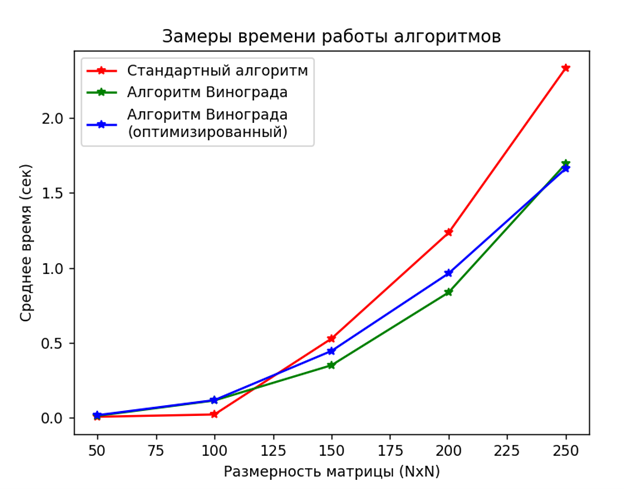
\includegraphics[width=1\textwidth]{img/graph_even.png}
    \caption{График времени работы алгоритмов в зависимости от чётных размерностей матриц}
    \label{fig:graph_even} % Метка для ссылки на картинку
\end{figure}

\begin{table}[H]
    \centering
    \caption{Таблица времени (сек) работы алгоритмов в зависимости от чётных размерностей матриц}
    \begin{tabular}{|l|c|c|c|c|c|}
        \hline
        \textbf{Алгоритм} & \textbf{50} & \textbf{100} & \textbf{150} & \textbf{200} & \textbf{250}\\
        \hline
        Стандартный & 0.0053 & 0.021 & 0.53 & 1.2 & 2.3 \\
        Винограда & 0.012 & 0.11 & 0.35 & 0.84 & 1.7 \\
        Винограда (оптимизированный) & 0.016 & 0.12 & 0.45 & 0.96 & 1.7 \\
        \hline
    \end{tabular}
    \label{table:table_even}
\end{table}

\begin{figure}[H]
    \centering
    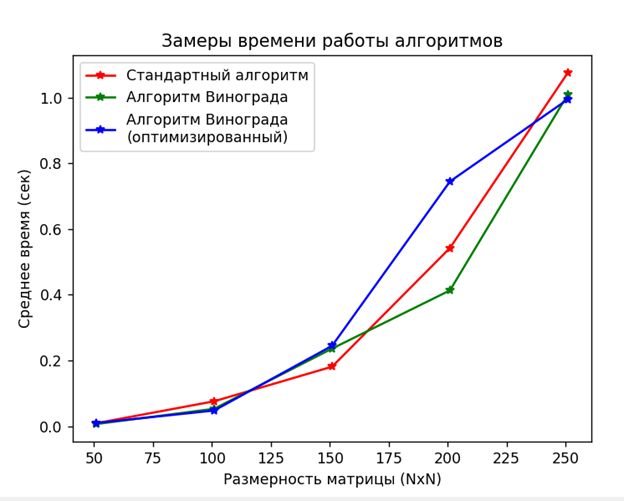
\includegraphics[width=1\textwidth]{img/graph_odd.png}
    \caption{График времени работы алгоритмов в зависимости от нечётных размерностей метриц}
    \label{fig:graph_odd} % Метка для ссылки на картинку
\end{figure}

\begin{table}[H]
    \centering
    \caption{Таблица времени (сек) работы алгоритмов в зависимости от нечётных размерностей матриц}
    \begin{tabular}{|l|c|c|c|c|c|}
        \hline
        \textbf{Алгоритм} & \textbf{51} & \textbf{101} & \textbf{151} & \textbf{201} & \textbf{251}\\
        \hline
        Стандартный & 0.0091 & 0.076 & 0.18 & 0.54 & 1.1 \\
        Винограда & 0.0066 & 0.053 & 0.24 & 0.41 & 1.0 \\
        Винограда (оптимизированный) & 0.01 & 0.048 & 0.24 & 0.74 & 0.99 \\
        \hline
    \end{tabular}
    \label{table:table_odd}
\end{table}

\subsection*{Вывод}

\hspace{1.25cm}
По проведённым исследованиям была выявлена большая скорость работы алгоритма Винограда над стандартным алгоритмом за счёт уменьшения трудоёмкости вычислений и чем больше размерность матрицы, тем больше видна разница в скорости алгоритмов. Однако на нечётных размерностях такого выигрыша не наблюдается за счёт дополнительного цикла, корректирующего вычисленное значение в алгоритме Винограда. Быстрее алгоритма Винограда работает его оптимизированная версия за счёт двоичного сдвига вместо умножения на 2, объединения III и IV частей алгоритма Винограда, выноса начальной итерации из каждого внешнего цикла, что уменьшает трудоёмкость.

\newpage